\documentclass[a4paper,12pt]{article}

\usepackage[backend=bibtex]{biblatex}
\usepackage{geometry}
\usepackage{titling}
\usepackage{titlesec}
\usepackage[english]{babel}
\usepackage[hidelinks]{hyperref}
\usepackage{listings}
\usepackage{xcolor}
\usepackage{graphicx}
\usepackage{forest}
\usepackage{tikz-qtree}
\usepackage{setspace}

\addbibresource{ref.bib}

\graphicspath{ {./images} }

\titleformat{\section}
{\Huge}
{}
{0em}
{}[\titlerule]
\geometry{a4paper,total={170mm,257mm},left=25mm,right=25mm,}

\author{Lucas Standen}
\title{Why FOSS software is preferred in the development and privacy space?}


\begin{document}
\maketitle

\newpage

\section{Using this document}
This document is written using the {\LaTeX} text compiler. The compiler has set up clickable links,
clickable references and a clickable table of contents, so please use these to your advantage. 
The Tex source and Bib Tex bibliography is available for all at 
\url{https://github.com/standenboy/epq/} under the MIT/X document license.

\tableofcontents
\newpage

\setlength{\parskip}{1em}

{\setlength{\parindent}{0cm}

\section{A brief introduction}

\section{Used language in this paper}
Throughout this paper I will use language specific to the field of computer science, and as such
it makes sense to provide a brief overview for those who don't know what specific terms mean.

\begin{description}
	\item[Licenses] In this setting a license is a legal document that is distributed with
		almost all modern software, which describes how someone can use a piece of software.
	\item[Free Software] This term refers to software under specific licenses, making them 
		free for the user to use (free as in freedom, not the monetary cost). This will
		be covered further in the next section.
	\item[Open Source] This term refers to a piece of software, where the original code for it
		is publicly available. This too will be covered further in the next section.
	\item[FOSS] An acronym for "\textbf{F}ree and \textbf{O}pen \textbf{S}ource \textbf{S}oftware".
\end{description}

\section{What is Free Software?}
The Free Software movement is one that has been active for over 40 years \cite{GNUmaifesto}, it has
created some of the most important tools in computing that are used by billions on a daily basis. 
It is so engraved in our lives, yet so few even know what the term means; In a simple note, it is
software for a computer, phone or other device that can be used without violating the users 
freedom.

The definition of what counts Free Software and what is software freedom can vary depending on who 
you ask, but it was originally written that software that allows the following freedoms is 
Free Software:

\begin{description}
	\item[0] The freedom to run a program for any purpose
	\item[1] The freedom to study how a program works, and modify it to your needs
	\item[2] The freedom to redistribute a piece of software
	\item[3] The freedom to redistribute a edited version of software publicly
\end{description}
\textit{These freedoms were written by Richard Stallman\cite{FOSSdef} who is ever 
	important in this space.}

It is important that one does not confuse Free Software with software that is monetarily free, 
this is known as Freeware. Free Software defends the users rights to use and modify software and
is not focused on its cost.

One should also note the differences between Free Software and Open Source software. In Open Source
software, like Free Software, the original code for a program is available to anyone, however
in Open Source, this is to better the projects development and usability, whereas in Free Software
it is to better the users freedom. They both use the same methods to achieve differing goals; this
often leads them to be commonly used together, as the benefits a user gets from Free Software is 
much the same in Open Source software, and vice versa.

The main goal of Free Software is to allow the user to have as much freedom as possible when using 
a piece of software for any purpose. This is in contrast to the traditional alternative, called
Proprietary Software, which can be defined as software that the user can not edit, modify or 
redistribute without the original publishers permission. This kind of software intentionally 
restricts the users freedom, usually for the purpose of profit or control of the software. Some 
common examples of Proprietary Software, are Microsoft's \textit{Windows}, Apple's \textit{iOS}, 
and Google's \textit{Chrome} web browser.

Many people don't know that they already use Free Software\cite{COMMONfoss}, but often the tools
they use most often are Free Software. A few examples of this are, Krita\cite{KRITA}; a graphics 
design and art tool that is used frequently in animation, and other digital art, is made and 
managed by the KDE foundation\cite{KDE}, who make exclusively Free Software. Dovecot\cite{DOVECOT}; 
an email server used by major email providers and is Free Software. A final example is 
Firefox\cite{FIREFOX} a Free Software web browser made by Mozilla that makes up 2.71\% of the 
browser market share as of 2024, however in the past has had up to 30\%\cite{BROWSERmarketshare}. These 
are all more modern examples of Free Software, however over the past 40 years, there have 
been countless others. 

\section{A brief history of FOSS}
The term Free Software was first coined by Richard Stallman in 1983\cite{GNUproject}, however even
before this, examples of Free Software (and the disapproval of Proprietary Software), were already
starting to show. 

One of the earliest examples of the disapproval of Non-Free Software, was the response to Microsoft's 
\textit{An open letter to hobbyists}, which was written by Bill Gates in 1976. This letter detailed 
that people had been stealing from Microsoft, as many people had brought hardware through 
them, but far fewer people had brought required software for said hardware. The fact this was happening 
at a scale large enough to cause this showed how many computing groups, also known as hacker groups/spaces, 
weren't willing to pay for the software they used, believing that if they brought the hardware they had done 
all that was needed\cite{OPENletter}. It is often believed that this is one of the first examples 
of \textit{hacker culture}, which would become more common into the 80's and 90's, and was the 
starting point of the current Free Software movement.

A key figure in \textit{hacker culture}, as previously mentioned, is Richard Stallman. In the 
 1980's he left his job at MIT to work full time on the GNU project, which was designed
to be a full recreation of AT\&T's Unix operating system from the ground up as Free Software. 
The idea was to allow anyone access to a Unix like machine without paying AT\&T's expensive license 
fees, and allow any user to view it, redistribute or edit; it was to be the first fully free 
operating system. The early development of GNU was relatively slow, and it was not a completely free 
system for many years, as some core parts of the operating system were missing, meaning Non-Free 
alternatives had to be used. However this would later change in 1991, when final additions would
be created.

In 1988 BSD Net1 would release\cite{BSDnet1}, this was the first fully open version of the Berkeley 
Software Distribution version of Unix. BSD was by no means new by this point, however it wasn't 
fully free until this point. It had completely rewritten all the code from the original 
Unix that previous versions contained, meaning it was now completely free from AT\&T's licenses.
It would be the start of a long linage of Open Source operating systems which are now the base
of MacOS, FreeBSD and OpenBSD and is often deamed as the first Open Source operating system.

The GNU project, while still not fully finished, saw the final piece of the puzzle when 
Linux\cite{LINUX} released in 1991, it was a fully free kernel which GNU was still lacking (however 
it did get its own kernel called GNU hurd but Linux is far more commonly used). With GNU and Linux 
paired together a user could finally get a fully free operating system for general use, this 
combination of software is still in use today, having a 4.7\% market share globally on desktop
computers\cite{LINUXmarket}, and on web servers it is dominant. In recent years it has also shown
some use in gaming, with it being the operating system used by Valves \textit{steam deck} gaming 
handheld\cite{STEAMdeck}.

Since Linux's release there haven't been as many major events in the space and more so a steady flow
of updates and new features, with a large jump over Covid. As of 2024 it would be hard not to 
say Free Software is fully viable against its Proprietary counterpart.

\section{How is Free Software developed?}
The process of developing Free Software has changed over time, especially as the internet came to be,
allowing developers from all across the world to add things. In modern terms the development process is 
very simple, a developer can look at a piece of code, make changes to a local version of it, then it 
can be uploaded to a central online version of the code, to be checked by lead maintainers, before becoming
the part of the main version (developers would say creating a local branch and submitting a pull request). 
This method was popularized by version control systems; such as git\cite{GIT}, which is also Free Software. 
What these tools allow for is the work of many people to brought together into one single code base.

When code is submitted, it generally gets split into individual chunks (called patches) which each
have an individual purpose. Each patch added will fix 1 bug or add 1 feature, this leads to a simple
development cycle that can easily be used to fix bugs, by breaking them down into small patches that
need to be written, and distributing the work between many developers. 

Without going into too much detail, this is done by merging all contributions into the main code base
by comparing line numbers in differing versions, this is a fully automated process, managed by your
version control system. This pattern of development is liked amongst programmers as it allows many 
to submit code all at once, which is invaluable if your project has many developers. This method
is also commonly used in Non-Free Software, to manage large development teams\cite{NONFREEvcs}.

\section{Comparing Free Software to its Proprietary counterparts}
As previously mentioned there are many different examples of Free Software, often made to be an 
alternative to a common piece of Proprietary software, each have their pro's and con's. To compare,
one can look at performance data and usability. To show a wide range of software, to compare this paper 
will look at programming IDE's, web browsers, and office software, as there make up a large amount 
of software, that are used by the majority of computer users.

\subsection{Programming IDE's}
\textit{An \textbf{IDE} is an \textbf{I}ntegrated \textbf{D}evelopment \textbf{E}nvironment}

The main IDE's used by developers are Free Software, but there are a few Non-Free ones that are used.
To compare text editors, one can look at \textit{Vs Code} as an example of open software, with 73\% of 
developers claiming to have used it at some point, and \textit{IntelliJ}, as an example of Non-Free 
software, with 26\% of developers claiming to have used it at some point\cite{IDEusage}.

These tools are both commonly used personally and professionally, and are of a similar size, making them
ideal to compare. On the performance side of the argument, VS Code has Intellij beat, being faster to open
and generally more lightweight than Intellij, this has been put up to the fact that VS Code is written in 
JavaScript, which is faster than Java, which is what Intellij is written in\cite{VSCODEvsintellij}.

On the usability side, things are more even, both editors have features that makes them better than each other,
each of them have plug-ins support, advanced text editing features and each have auto completion. However in this
sense VS Code still generally comes ahead, with its more main stream user base, more gets made for it, and as
it is Open Source easier for users to add features, in the for of patches, and in the form of plug-ins, although
no definite numbers are available on exact plug-in counts publicly, VS Code is most defiantly ahead.

\subsection{Web Browsers}
To compare web browsers, one can look at two commonly used browsers, Google Chrome, and Firefox. Both of these
are known projects, that are used by billions every day, one can look at their performance and usability to compare
these projects. 

\begin{figure}[h]
	\caption{Comparing speed of browsers, time \textit{(lower is better)}}
	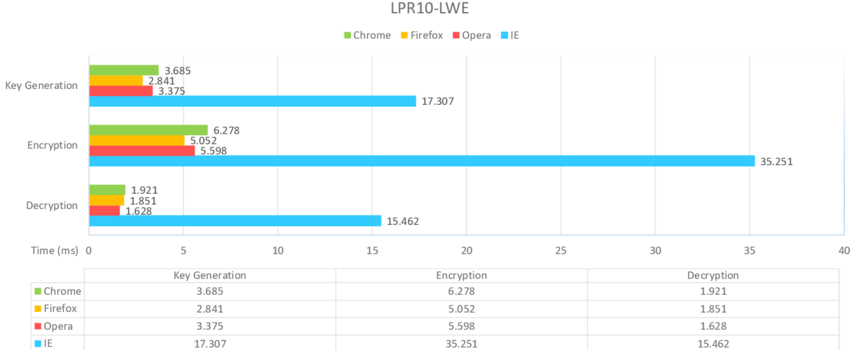
\includegraphics[width=\textwidth]{webbrowserperfomace.png}
	\center{\cite{BROWSERperformace}}
\end{figure}

This graph denotes each browsers performance in encryption and decryption, while not fully representative of all use 
cases, it is one of many things that goes into the final speed of the browser. As the graph shows, Firefox's FOSS 
implementation of JavaScript has lead to a faster final product, most likely as more people have had eyes on the code, 
and suggested optimizations over the past 20 years. On the front of performance it is clear that the FOSS tool has beaten 
the Proprietary counterpart.

In respect to usability things come more to user preference, so what one needs to look at, is customizability; the ability 
to make a piece of software exactly fit their needs. In this yet again Firefox wins out, while both Firefox and Google Chrome 
have plug-in capability's, Firefox is known for its completely open system to them, allowing any and all extensions to be
used. In contrast google limits what can be used via the "manifest" documents, this series of documents describes what is
and isn't allowed in the Chrome browser, and is significant as it holds a large market share. The most recent one of these
documents, manifest V3\cite{MANIFESTv3}, has come under many eyes, as it will disallow ad blockers, and other extensions that selectively
remove content from web pages.

In today's world, the majority of browsers are based on Chrome in some way or another with Firefox being one of the few exceptions 
to this rule. Due to this, most browsers will be effected by manifest V3 as it comes into full effect in the coming years.
As this happens it will become increasingly hard to deny that Firefox is easier to customize and make usable to the users needs.

\subsection{Office Software}
When looking at office software, their are two commonly used tools, Microsoft Office (also known as 365), and Libreoffice.
Microsoft Office is Proprietary software, and has been since its creation in the early days of personal computing, Libreoffice 
on the other hand, has been FOSS software from the start (libre actually means free in spanish, so this is no surprise). 
They both provide advanced features, and for the most part are completely cross compatible. In this sense they have become
almost identical tools. 

As the tools are so similar one will find it's not worth comparing them, in this way we can say that there is no difference,
they are both mature, well used, effective suites of software, they are equal. This is something many people struggle to 
see sometimes as they have been using one piece of Non-Free software for so long, they don't want to move to anything else.
This has negative effects on the users, many Non-Free tools are effected by cyber attacks, and long lasting bugs, that could 
be fixed by switching to Free Software alternatives, which are now at an equal state to the alternative.

\subsection{General conclusions}
Overall one can see that in many areas of software use, FOSS tools are already at an equal state or better, than the Non-Free
counterparts, for general users. One may find that this balance begins to change in more specific fields, where optimisation and
speed may become more important than it is to the common computer user.

\section{What makes Free Software so appealing to developers?}
\section{What makes Free Software so appealing to privacy experts?}
\section{Where else is Free Software used and why?}
\section{What's next for the Free Software space?}
\section{Final thoughts}

\newpage
\printbibliography
}
\end{document}
